\documentclass[smallcondensed,final]{svjour3}                     % onecolumn (standard format)
%\documentclass{article}
\RequirePackage{fix-cm}

\usepackage{graphicx}
\usepackage[fleqn]{amsmath}
\usepackage{amssymb}
\usepackage{bm}
%\usepackage{pgf}
%\usepackage[polutonikogreek]{babel}

\begin{document}

\title{Symbolic linearization of equations of motion of constrained multibody systems}

\titlerunning{Symbolic linearization of equations of motion of constrained multibody systems}        % if too long for running head

\author{Dale L. Peterson\and Gilbert Gede\and Mont Hubbard}

\institute{Dale L. Peterson, Gilbert Gede, Mont Hubbard \at
           Sports Biomechanics Laboratory\\
           Department of Mechanical and Aerospace Engineering\\
           University of California Davis\\
           Davis, CA 95616-5294\\
           Tel.: +1 530 752 2163\\
           \email{\{dlpeterson,ggede,mhubbard\}@ucdavis.edu}}

\date{Received: date / Accepted: date}

\maketitle

\begin{abstract}
% Context
Many common dynamic mechanical systems are subject to configuration or velocity
constraints.
% Need  (what we have and what we want)
Analyses of such systems often require linearized forms of the motion
equations.
% Task
To address this issue, we developed a procedure for organizing the constraint
and motion equations and their subsequent linearization.  This procedure was
specifically developed for equations of motion generated by Kane's method, but
is compatible with any method as long as the following are true: only ordinary
differential equations are required to describe the system, and independent and
dependent states remain in the final equations (i.e. no DAE's, dependent
variables are not substituted away).
% Object of the document
Following a brief review of Kane's method and the structure of the equations it
generates, we present the procedure to symbolically linearize the nonlinear
motion equations of constrained multibody systems, and illustrate it with an
example of the rolling disk.

\keywords{linearization, constrained multibody systems, symbolic dynamics, control}
\end{abstract}

\section{Introduction}
\label{sec:intro}
Design of linear state feedback controllers and first order stability analysis
of equilibria are two of the most common uses of multibody system dynamics
models. Both of these uses require linearized equations of motion. For
unconstrained systems, obtaining the linearized equations of motion is as
simple as arranging the equations of motion in first order form ($\dot{x} =
f(x, t)$) and evaluating the Jacobian of the right hand side function, with
respect to the states, evaluated at the equilibria point of interest.  However,
when the system in questions has constraints, i.e., not all the states are
independent, this process is not as straightforward.

For a system with constraints, Kane's dynamical equations\cite{Kane1985} are
first order ODE's (in the generalized speeds) which include both the
independent and dependent states (assuming the dependent states have not been
algebraically eliminated). The kinematical and dynamical differential equations
can be solved for the time derivatives of the generalized coordinates and
generalized speeds, respectively. Taken together, it is tempting to think that
this system of first order differential equations could be linearized in the
same fashion as an unconstrained system.  Unfortunately, this is not the case.
Linearizing these equations in the same manner as one would for an
unconstrained system (by directly computing the Jacobian) is incorrect and will
yield incorrect linearized equations (and subsequently incorrect eigenvalues,
in the case of a stability analysis). We illustrate this by means of a familiar
example, the rolling disk, formulated with a non-traditional set of coordinates
and generalized speeds which are not all independent. We provide a systematic
method to correctly generate the linear equations of motion for constrained
systems which have been found using Kane's method (or any other method which
results in equations with the same form). We apply this method to the rolling
disk example to illustrate that it yields eigenvalues that match previously
published results.

We consider three levels of constraints: configuration, velocity, and
acceleration. Configuration (holonomic) constraints limit the location or
orientation of parts of the system, relative to the external world or other
parts of the system. Velocity (nonholonomic of time differentiated holonomic)
constraints limit the speeds at which the configuration can change.
Velocity constraints most often appear in systems where there is rolling
without slip or there are closed kinematic loops. For this procedure,
acceleration level constraints are assumed to be time differentiated velocity
constraints.

% TODO: Improve literature review.
Bottema appears to be the first author to have shown that special
considerations are needed for linearizing nonholonomic systems
\cite{Bottema1949}. While other authors have examined linearization of
nonholonomic systems, we have found that most techniques are not directly
applicable to equations formed using Kane's method, and while we do not doubt
that they \textit{could} be applied correctly, the details of how to do so, as
far as the authors are aware, have not been explicitly presented. Kang et al.
\cite{Kang2003} and Negrut and Ortiz \cite{Negrut2006} have both explored
linearization, but these methods have been developed for equations of motion
found using Lagrange's method, which contain Lagrange multipliers (which are
not present in equations of motion generated from Kane's method). Further, both
of these papers lack a discussion of basic concepts such as how many quantities
are independent, and in the case of eigenvalue computation, how many
eigenvalues should be present. Minaker and Rieveley \cite{Minaker2010} and
Schwab and Meijaard \cite{Schwab2003} both have developed techniques for
generating equations of motion (and linear forms thereof) using Lagrange's
method; the work of Schwab and Meijaard can be applied symbolically while
Minaker and Reiveley's approach is numeric in nature. Neither discuss the
choice of generalized speeds as in Kane's method: both form the equations of
motion in terms of second time derivatives of the coordinates.  Further,
neither of these works address constraints which cannot be eliminated (e.g.,
nonlinear configuration constraints), nor do they address what approach should
be taken when a single choice of dependent states may not suffice. While
Neuman presents a symbolic (as opposed to numeric) formulation for
linearization of the Q-matrix formulation of the Lagrangian\cite{Neuman1984},
his work makes no mention of constrained systems and attempts to contact the
author regarding the software (algebraic robot modeler -- Arm) as well as
internet searches for the software have been fruitless.

% What does it mean for the equations to be symbolic/analytic in nature?

% TODO:reiterate limitations of model
This paper presents linear, first order differential equations relating the
time derivatives of \textit{all} speeds and coordinates to the independent
speeds and coordinates, for any point of linearization.  A provided example
demonstrates the necessity of these equations.  We demonstrate how a reduced
portion of these linearized equations can be used to perform standard stability
analysis (i.e., for control system design or linear stability analysis).  The
formalism presented here is generic enough to cover most examples of
time-varying constrained multibody systems with arbitrary external inputs and
arbitrary specified quantities.
% TODO: electronic supplementary material with examples for other methods
% TODO: rewrite following sentences after e.s.m.
The procedure was created for systems whose equations of motion have been
derived with Kane's method. Although also applicable to dynamic system
equations formulated using other methods, it is restricted to systems which can
be completely described by a set of ODE's (i.e., DAE's needn't be solved).

We begin with a review of Kane's method for generating equations of motion is
reviewed first, in order to properly orient the reader to the format and some
of the qualities of the generated equations. Next, we apply Kane's method to
generate the equations of motion for the rolling disk, but we purposefully
introduce a dependent coordinate and three dependent speeds in the formulation.
The need for a different linearization technique is demonstrated with this
example. In response to this need, we present the newly developed linearization
procedure and its derivation. This new linearization procedure is applied the
same rolling disk example to illustrate its validity and an example of its
application. Finally, we discuss other details and nuances of the procedure and
its use, as well as directions for future work.

\section{Kane's Method, briefly}
\label{sec:kane_method}
To familiarize the reader with Kane's method, some concepts relating to its use
will be described.  The first is the use of generalized speeds in addition to
generalized coordinates.  The second concept is in how these generalized speeds
can be used to project permissible motions of the system, and how this removes
the need to consider non-contributing (internal constraint) forces.  Then, the
mathematical steps required to use Kane's method are shown and described.

When using Lagrange's method, generalized coordinates are used to describe the
configuration of a system while the time derivatives of the generalized
coordinates describe the velocities of a system.  Kane's method allows for the
velocities of a system to be written in terms of generalized speeds, which are
not required to be the time derivatives of coordinates (although such a
definition is permitted).

The benefit of choosing generalized speeds to be other than simply the
derivatives of the corresponding generalized coordinates can be seen in the
following example. If the orientation of a rigid body were to be described
using using Euler parameters or quaternions as coordinates, its angular
velocity in terms of time derivatives of those coordinates is relatively
complicated; it also requires a velocity constraint. Using generalized speeds
allows for the angular velocity to be expressed more simply as
\begin{align}
\label{eq:ex1}
{^N}\bar{\omega}^B = u_1 \hat{b}_1 + u_2 \hat{b}_2 + u_3 \hat{b}_3
\end{align}
or, the angular velocity of rigid body $B$ in the reference frame $N$ is the
defined as the sum of three generalized--speed basis--vector products.
The derivatives of these generalized speeds will appear in the equations
of motion, rather than the twice time differentiated generalized coordinates
($\ddot{\mathbf{q}}$'s).

A drawback of allowing such definitions can be seen when formulating the
kinematic differential equations, which relate the rate of change of the
generalized coordinates to the generalized speeds. These equations become more
complicated (in comparison to $\dot{q}_i = u_i$), but this is usually offset by
the significantly simpler dynamical equations of motion~\cite{Mitiguy1996}.

Use and understanding of Kane's method requires the use and understanding of
partial velocities and partial angular velocities. These are simply the
partial derivatives of the (angular) velocity vectors with respect to the
generalized speeds. For example, for the angular velocity in equation
(\ref{eq:ex1}), the partial angular velocities of body $B$ in reference frame
$N$ are
\[
{^N}\bar{\omega}^B_{1} = \hat{b}_1 \quad \quad
{^N}\bar{\omega}^B_{2} = \hat{b}_2 \quad \quad
{^N}\bar{\omega}^B_{3} = \hat{b}_3
\]
and it can be seen that the partial velocities represent the direction of
motion associated with each generalized speed. The geometric interpretations of
these partial (angular) velocities are discussed at length by
Lesser\cite{Lesser1992}.

Taking the dot product of each partial velocity and both sides of Newton's
second law, $\bar{F}=m\bar{a}$ (or the rotational equivalent), only terms that
are parallel to the partial velocities remain; one scalar equation is generated
for each generalized speed. An important byproduct is that internal constraint forces
(non-contributing forces) imposed by objects such as pin or sliding joints no
longer need to be considered. The reason for this is that partial velocities
are \textit{by construction} perpendicular to forces of constraint. Constraint
forces can be included in the formulation, but will not appear in the final
equations of motion because of this very desirable property.

In summary, Kane's method allows for velocities to be defined in terms of
generalized speeds, allowing for simpler velocity expressions.  The dot product
of each partial velocity (the direction of motion associated with each
generalized speed) with Newton's second law (or Euler's equations) removes all
terms which are not related to the rate of change of each generalized speed.
This generally results in simple equations of motion, which are easier to form.

The mathematical formalism for applying Kane's method to multibody systems
follows. Consider a system composed of particles $P_1,...,P_h$, rigid bodies
$B_1,...,B_g$, with points of force application $Q_1,...,Q_k$, and reference
frames of torque application $E_1,...,E_c$, all defined relative to the
inertial reference frame $N$. This system has generalized coordinates
$q_1,...,q_n$ and generalized speeds $u_1,...,u_o$.  While it common that $n =
o$, this is not a requirement when using Kane's method. Additionally, there are
$l$ configuration constraints and $m$ velocity constraints.

In order to properly apply Kane's method, the velocities of each component in
the system need to be written as linear combinations of the generalized speeds.
The translational velocity of the particles are
\begin{align}
\label{eq:particle_translational}
{^N}\bar{v}^{P_i} = \sum^o_{j=1} {^N}\bar{v}^{P_i}_{j} u_j + {^N}\bar{v}^{P_i}_t
\quad \quad i=1,...,g
\end{align}
while the translational velocity of rigid body mass centers are
\begin{align}
\label{eq:rb_translational}
{^N}\bar{v}^{B_i^*} = \sum_{j=1}^o {^N}\bar{v}^{B_i^*}_{j} u_j +
{^N}\bar{v}^{B_i^*}_t \quad \quad i=1,...,h
\end{align}
and finally the translational velocity of points which have applied forces are
\begin{align}
\label{eq:points_translational}
{^N}\bar{v}^{Q_i} = \sum_{j=1}^o {^N}\bar{v}^{Q_i}_{j} u_j + {^N}\bar{v}^{Q_i}_t
\quad \quad i=1,...,k
\end{align}
Next, the angular velocity of rigid bodies are
\begin{align}
\label{eq:rb_rotational_bodies}
{^N}\bar{\omega}^{B_i} = \sum_{j=1}^o {^N}\bar{\omega}^{B_i}_{j} u_j +
{^N}\bar{\omega}^{B_i}_t \quad \quad i=1,...,h
\end{align}
and the angular velocity of reference frames which have applied torques are
\begin{align}
\label{eq:rb_rotational_frames}
{^N}\bar{\omega}^{E_i} = \sum_{j=1}^o {^N}\bar{\omega}^{E_i}_{j} u_j +
{^N}\bar{\omega}^{E_i}_t \quad \quad i=1,...,c
\end{align}

In these equations, each term $\bar{v}_t$ or $\bar{\omega}_t$ represents a
velocity or angular velocity component which is a prescribed function of time,
and has no dependence on generalized speeds (e.g., a motor or crank driven at a
specified rate).

For this system, we consider configuration constraints of the form
\begin{align}
\label{eq:configuration_constraints}
\mathbf{f}_c(\mathbf{q}, t) = \mathbf{0}
\end{align}
where the terms $\mathbf{f}_c$ and $\mathbf{0}$ have the shape $l \times 1$.
The velocity constraints are taken to have the form
\begin{align}
\label{eq:velocity_constraints}
\mathbf{f}_v(\mathbf{q}, \mathbf{u}, t) = \mathbf{0}
\end{align}
where the terms $\mathbf{f}_v$ and $\mathbf{0}$ have the shape $m \times 1$,
and $\mathbf{f}_v$ depends linearly on $\mathbf{u}$.  It is important that the
velocity constraints include the time-differentiated configuration constraints
or equivalent constraints which produce the same behavior. Furthermore,
velocity constraints should be written such that generalized speeds and
coordinates appear, but $\dot{\mathbf{q}}$ terms do not.  Finally, acceleration
constraints are typically time-differentiated velocity constraints (or
similarly formed from kinematic considerations) and are assumed to have the
form
\begin{align}
\label{eq:acceleration_constraints}
\mathbf{f}_a(\mathbf{q}, \dot{\mathbf{q}}, \mathbf{u}, \dot{\mathbf{u}}, t) =
\mathbf{0}
\end{align}
In contrast to the velocity constraints, our formulation permits the
acceleration constraints to involve $\dot{\mathbf{q}}$ terms (alternatively
they can be eliminated by appealing to the kinematic differential equations).

By assumption, the velocity constraints are linear with respect to
$\mathbf{u}$, so we introduce
\begin{align}
\label{eq:constraint_B}
\mathbf{B} &\triangleq \nabla_{\mathbf{u}} \mathbf{f}_v (\mathbf{q}, \mathbf{u},
t)
\end{align}
which implies
\begin{align}
\label{eq:constraint_Bu0}
\mathbf{B}\mathbf{u} + \mathbf{f}_{vt}(\mathbf{q}, t) &= \mathbf{0}
\end{align}
where $\mathbf{f}_{vt}$ arises from explicit time varying terms that occur in
the velocity constraints. These typically arise from specified quantities whose
dynamics are being ignored (e.g., a motor spinning at constant speed).

With these definitions established, Kane's method can be applied. In vector
form, Kane's dynamical equations are
\begin{align}
\label{eq:kanes_eq}
\mathbf{F} + \mathbf{F}^* = \mathbf{0}
\end{align}
where $\mathbf{F}$ are the generalized active forces and $\mathbf{F}^*$ are the
generalized inertia forces. If Newton's second law is written as $f - ma = 0$,
$\mathbf{F}$ is the multibody generalization of $f$ and $\mathbf{F}^*$ is the
multibody generalization of $-ma$. As will be shown, these forces are obtained
by taking the dot product of the partial velocities/angular-velocities, as
defined in (\ref{eq:particle_translational}) - (\ref{eq:rb_rotational_frames}),
with the resultant forces/torques ($\bar{R}$/ $\bar{T}$) and with inertial
forces/torques ($\bar{R}^*$/$\bar{T}^*$).

The resultant force at a point is defined as the sum of all force vectors
acting directly on that point. The resultant torque on a reference frame is
defined similarly -- it is the sum of all torque vectors acting on that
reference frame. Distance forces do not need to be transformed into a resultant
force/torque pair for any components of the system; they only need to be
considered at the point of application (e.g., if a force $\bar{f}$ is the only
force applied to body $B$ at point $Q$, then $\bar{R}_{B^*}=0$ and
$\bar{T}_B=0$ but $\bar{R}_Q=\bar{f}$). The generalized active forces are
\begin{equation}
\label{eq:definition_F}
\mathbf{F} =
\begin{bmatrix}
\displaystyle \sum_{i=1}^g \bar{R}_{B^*_i} \cdot {^N}\bar{v}^{B^*_i}_1 +
\sum_{i=1}^h \bar{R}_{P_i} \cdot {^N}\bar{v}^{P_i}_1 +
\sum_{i=1}^k \bar{R}_{Q_i} \cdot {^N}\bar{v}^{Q_i}_1 +
\sum_{i=1}^g \bar{T}_{B_i} \cdot {^N}\bar{\omega}^{B_i}_1 +
\sum_{i=1}^c \bar{T}_{E_i} \cdot {^N}\bar{\omega}^{E_i}_1 \\
\displaystyle \sum_{i=1}^g \bar{R}_{B^*_i} \cdot {^N}\bar{v}^{B^*_i}_2 +
\sum_{i=1}^h \bar{R}_{P_i} \cdot {^N}\bar{v}^{P_i}_2 +
\sum_{i=1}^k \bar{R}_{Q_i} \cdot {^N}\bar{v}^{Q_i}_2 +
\sum_{i=1}^g \bar{T}_{B_i} \cdot {^N}\bar{\omega}^{B_i}_2 +
\sum_{i=1}^c \bar{T}_{E_i} \cdot {^N}\bar{\omega}^{E_i}_2 \\
\displaystyle \vdots \\
\displaystyle \sum_{i=1}^g \bar{R}_{B^*_i} \cdot {^N}\bar{v}^{B^*_i}_o +
\sum_{i=1}^h \bar{R}_{P_i} \cdot {^N}\bar{v}^{P_i}_o +
\sum_{i=1}^k \bar{R}_{Q_i} \cdot {^N}\bar{v}^{Q_i}_o +
\sum_{i=1}^g \bar{T}_{B_i} \cdot {^N}\bar{\omega}^{B_i}_o +
\sum_{i=1}^c \bar{T}_{E_i} \cdot {^N}\bar{\omega}^{E_i}_o
\end{bmatrix}
\end{equation}

We now define the inertia forces and torques, $\bar{R}^*$ and $\bar{T}^*$. We
leave out the inertial frame $N$ from the expressions; it is assumed to be $N$.
The inertia force for particle $P$ is
\begin{align}
\label{eq:particle_gen_inertia}
\bar{R}^*_P \triangleq -m_P {^N}\bar{a}^P
\end{align}
while the inertia force and inertia torque for rigid body $B$ is
\begin{align}
\label{eq:rb_translational_gen_inertia}
\bar{R}^*_{B^*} &\triangleq -m_B {^N}\bar{a}^{B^*} \\
\label{eq:rb_rotational_gen_inertia}
\bar{T}^*_B &\triangleq -{^N}\bar{\alpha}^B \cdot \bar{\bar{I}}^{B/B^*} -
{^N}\bar{\omega}^B \times \bar{\bar{I}}^{B/B^*} \cdot {^N}\bar{\omega}^B
\end{align}
Where $\bar{\bar{I}}^{B/B^*}$ is the central inertia dyadic of the rigid body
$B$ about its mass center $B^*$ \cite{Kane1985}. The generalized inertia forces
are
\begin{equation}
\label{eq:definition_Fstar}
\mathbf{F}^* =
\begin{bmatrix}
\displaystyle \sum_{i=1}^g \bar{R}^*_{B^*_i} \cdot {^N}\bar{v}^{B^*_i}_1 +
\sum_{i=1}^h \bar{R}^*_{P_i} \cdot {^N}\bar{v}^{P_i}_1 +
\sum_{i=1}^g \bar{T}^*_{B_i} \cdot {^N}\bar{\omega}^{B_i}_1 \\
\displaystyle \sum_{i=1}^g \bar{R}^*_{B^*_i} \cdot {^N}\bar{v}^{B^*_i}_2 +
\sum_{i=1}^h \bar{R}^*_{P_i} \cdot {^N}\bar{v}^{P_i}_2 +
\sum_{i=1}^g \bar{T}^*_{B_i} \cdot {^N}\bar{\omega}^{B_i}_2 \\
\displaystyle \vdots \\
\displaystyle \sum_{i=1}^g \bar{R}^*_{B^*_i} \cdot {^N}\bar{v}^{B^*_i}_o +
\sum_{i=1}^h \bar{R}^*_{P_i} \cdot {^N}\bar{v}^{P_i}_o +
\sum_{i=1}^g \bar{T}^*_{B_i} \cdot {^N}\bar{\omega}^{B_i}_o
\end{bmatrix}
\end{equation}

All the terms in (\ref{eq:kanes_eq}) are now defined, but this equation is
valid only if there are no velocity constraints. If there are velocity
constraints, the equations must be transformed. As we present them, Kane's
nonholonomic dynamical equations will be of dimension $o - m$, where $o$ is the
total number of generalized speeds and $m$ is the number of velocity
constraints. However, these $o-m$ equations generally involve all $o$ speeds
(we assume the dependent speeds and their time derivatives have \textit{not}
been algebraically eliminated). In order to obtain the nonholonomic dynamical
equations, however, a choice must be made as to which speeds will be dependent.
The methods for doing this are outside the scope of this paper, but it is
important that whatever selection is made avoids singularities which can occur
in certain configurations or sets of system parameters. For a careful treatment
of this, we encourage the reader to examine the work of Reckdahl
\cite{Reckdahl1996}.

We assume the $o$ generalized speeds are ordered $\mathbf{u} = [\mathbf{u}_i,
\mathbf{u}_d]^T$, where $\mathbf{u}_i\in\mathbf{R}^{o-m}$ and
$\mathbf{u}_d\in\mathbf{R}^{m}$ are the independent and dependent speeds,
respectively. The velocity constraint Jacobian matrix $B$ can be similarly
rearranged as $\mathbf{B} = [\mathbf{B}_i, \mathbf{B}_d]$, where
$\mathbf{B}_i\in \mathbf{R}^{m \times o-m}$ and $\mathbf{B}_d \in \mathbf{R}^{m
\times m}$. With this in mind, equation (\ref{eq:constraint_Bu0}) can be
written as
\begin{align}
\mathbf{B}_i \mathbf{u}_i + \mathbf{B}_d \mathbf{u}_d + \mathbf{f}_{vt}(\mathbf{q}, t) &= \mathbf{0} \\
\implies \mathbf{u}_d &= -\mathbf{B}_d^{-1} \mathbf{B}_i \mathbf{u}_i - \mathbf{f}_{vt}(\mathbf{q}, t)
\end{align}
For convenience, we define
\begin{align}
\label{eq:constraint_A}
\mathbf{A} \triangleq - \mathbf{B}_{d}^{-1} \mathbf{B}_i
\end{align}
and note that $\mathbf{A}\in\mathbf{R}^{m \times (o - m)}$. To constrain the
generalized active and inertia forces, we partitioned them in a similar
manner
\begin{align}
\label{eq:F_Fstar_rewrite}
\mathbf{F} = \begin{bmatrix} \mathbf{F}_i \\ \mathbf{F}_d \end{bmatrix} \quad
\quad \mathbf{F}^* = \begin{bmatrix} \mathbf{F}^*_i \\ \mathbf{F}^*_d
\end{bmatrix}
\end{align}
allowing the nonholonomic generalized forces to be written:
\begin{align}
\label{eq:F_Fstar_nonholonomic}
\tilde{\mathbf{F}} = \mathbf{F}_i + \mathbf{A}^T \mathbf{F}_d \quad \quad
\tilde{\mathbf{F}}^* = \mathbf{F}_i^* + \mathbf{A}^T \mathbf{F}_d^*
\end{align}
which allows Kane's nonholonomic dynamical equations to be written as
\begin{align}
\label{eq:kanes_eq_nonholonomic}
\tilde{\mathbf{F}} + \tilde{\mathbf{F}}^* = \mathbf{0}
\end{align}
This process of constraining the equations of motion reduces the number of
equations from $o$ to $o-m$. However, the (\ref{eq:kanes_eq_nonholonomic}) still
contain $o$ unknowns ($\dot{\mathbf{u}}_1,...,\dot{\mathbf{u}}_o$). By
augmenting (\ref{eq:kanes_eq_nonholonomic}) with the acceleration constraint
equations (\ref{eq:acceleration_constraints}), we obtain $o$ equations in
$o$ unknowns. Note that equations (\ref{eq:kanes_eq_nonholonomic}) and
(\ref{eq:acceleration_constraints}) are linear in the $\dot{u}_i$'s. The
augmented system of equations is
\begin{align}
\label{eq:F_Fstar_f_a}
\begin{bmatrix}
\tilde{\mathbf{F}} + \tilde{\mathbf{F}}^* \\
\mathbf{f}_a (\mathbf{q}, \dot{\mathbf{q}}, \mathbf{u}, \dot{\mathbf{u}}, t)
\end{bmatrix} = \mathbf{0}
\end{align}

For convenience, we summarize the critical equations in Table
\ref{table:assumptions}.

% This is incomplete unless we mention the kinematic equations so I am leaving
% it out for now. I think we have stated this earlier.
%With regards to obtaining linearized equations, it is
%critical to note that solving equations (\ref{eq:F_Fstar_f_a}) for the
%$\dot{\mathbf{u}}$'s, 
%with respect to $\mathbf{u}_i$ does not give the correct linear equations. The
%reasons for this will be covered later.

%TODO: Expand on r (exogenous inputs)
\begin{table}[htbp]
  \centering
  \caption{Constrained multibody system governing definitions and equations}
  \label{table:assumptions}
  \begin{tabular}[c]{l l l}
    Quantity & Shape & Description\\
    \hline
    $\bm{q},\bm{\dot{q}}$ & $\mathbf{R}^n$ & Coordinates and their time
    derivatives\\
    $\bm{u}, \bm{\dot{u}}$ & $\mathbf{R}^o$ & Speeds and their time derivatives\\
    $\bm{r}$ & $\mathbf{R}^s$ & Exogenous inputs \\
  \end{tabular}
  \begin{tabular}[c]{r @{ $=$ } l l}
    \multicolumn{3}{c}{ } \\
    \multicolumn{2}{c}{Equation} & Description \\
    \hline
    $\bm{f}_{c}(\bm{q}, t)$ & $\bm{0}_{l \times 1}$ & Configuration level constraints \\
    $\bm{f}_{v}(\bm{q}, \bm{u}, t)$ & $\bm{0}_{m \times 1}$ & Velocity level constraints \\
    $\bm{f}_{a}(\bm{q}, \bm{\dot{q}}, \bm{u}, \bm{\dot{u}}, t)$ & $\bm{0}_{m
    \times 1}$ & Acceleration level constraints \\
    $\bm{f}_{0}(\bm{q}, \bm{\dot{q}}, t) + \bm{f}_{1}(\bm{q}, \bm{u}, t)$ &
    $\bm{0}_{n \times 1}$ & Kinematic differential equations \\
    $\bm{f}_{2}(\bm{q}, \bm{\dot{u}}, t) + \bm{f}_{3}(\bm{q}, \bm{\dot{q}},
    \bm{u}, \bm{r}, t)$ & $\bm{0}_{(o - m) \times 1}$ & Dynamic differential equations
  \end{tabular}
\end{table}

Not all of the $n$ generalized coordinates are independent due to the $l$
configuration level constraints (e.g., holonomic constraints resulting from
closed kinematic loops). Similarly, not all of the $o$ generalized speeds are
independent due to the $m$ velocity level constraints.  Velocity level
constraints result from time differentiated configuration constraints or
nonholonomic constraints (e.g., no-slip rolling).  The $m$ acceleration level
constraints are assumed to be obtained by time differentiating the $m$ velocity
level constraints.  Just as Kane's method does not require $n = o$,
neither does our linearization procedure. The $s$ exogenous inputs include
control system inputs and/or external disturbance forces or torques applied to
the system.

The kinematic differential equations are organized into the quantities
$\mathbf{f}_0$ and $\mathbf{f}_1$; terms depending upon $\dot{\mathbf{q}}$ are
placed into $\mathbf{f}_0$, all other terms are placed into $\mathbf{f}_1$.
Similarly, the dynamic differential equations are organized into the
quantities $\mathbf{f}_2$ and $\mathbf{f}_3$; terms depending upon
$\dot{\mathbf{u}}$ are placed into $\mathbf{f}_2$, all other terms are placed
into $\mathbf{f}_3$. The motivation for this organizational scheme will be made
apparent in Section \ref{sec:derivations}.


\section{Dynamics Example}
\label{sec:example}
To illustrate Kane's method in the presence of configuration and velocity
constraints, we consider a thin disk $C$ rolling without slip on a horizontal
plane. The dextral unit vectors $\hat{c}_x, \hat{c}_y, \hat{c}_z$ are fixed to $C$
with $\hat{c}_y$ perpendicular to the disk plane. Let $r$ and $m$ be the
disk radius and mass, and assume a thin disk mass distribution so that
$I_{xx}=I_{zz}=mr^2/4$ and $I_{yy} = mr^2/2$. Take the inertial (Newtonian)
frame $N$ to be similarly equipped with dextral unit vectors $\hat{n}_x,
\hat{n}_y, \hat{n}_z$, with $\hat{n}_z$ perpendicular to the ground plane
(downwards) and aligned with the local gravitational field. To orient the disk,
first align $C$ with $N$, then apply successive body fixed ZXY rotations:
yaw $q_1$, roll $q_2$, and spin $q_3$.  Denote by $A$ and $B$ the two frames
associated with the first two intermediate rotations in the sequence; we refer
to these as the instantaneous yaw and lean frames, respectively. The unit
vector, $\hat{b}_z$ fixed in the $B$ frame, is parallel to the disk plane and
aligned with the position vector from the disk center $C^*$ to the lowest point
of the disk $P^*$. Figure \ref{fig:rolling_disc} shows how the generalized
coordinates are used to configure the disc.

\begin{figure}[!htb]
    \centering
    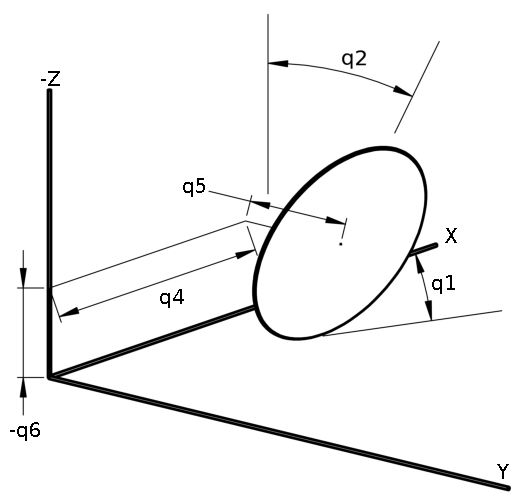
\includegraphics[width=0.8\textwidth]{disk_drawing_cropped.pdf}
    \caption{Configuration of rolling disc using non-minimal coordinates.}
    \label{fig:rolling_disc}
\end{figure}

Traditionally, to locate the center of the disk $C^*$ relative to the inertial
origin $N^*$, two coordinates are used to locate the contact point in the
ground plane; these two coordinates and the lean angle and yaw angles determine
the location of the center of the disk. The advantage of this approach is that
by using a minimal set of coordinates, the holonomic ground contact constraint
is always satisfied and hence no holonomic constraint equation is needed.

To illustrate how dependent coordinates must be
accounted for when linearizing the equations of motion, we purposefully locate
the center of the disk $C^*$ relative to the inertial origin $N^*$ with a
non-minimal choice of coordinates
\begin{equation*}
  \bar{r}^{C^*/N^*} = q_4 \hat{n}_x + q_5 \hat{n}_y + q_6 \hat{n}_z
\end{equation*}
which results in the configuration constraint $\mathbf{f}_c$
\begin{equation}
  \label{rd:f_c}
  rc_2 + q_6 = 0
\end{equation}
which must be satisfied for the disk to remain in contact with the ground.
While this constraint is easily avoided by appropriate choice of coordinates,
it serves to illustrate considerations which must be made when analyzing
systems in which there is no obvious way to eliminate configuration constraints.

Again to demonstrate how velocity constraints must be accounted for when
obtaining linearized equations of motion, we define the velocity of $C^*$ in
$N$ with a non-minimal choice of speeds, defined in the body-fixed ($C$) frame.
The angular velocity of $C$ in $N$, however, is defined in the intermediate
lean frame $B$.
\begin{align}
  \label{v_u}
  {^N}\bar{v}^{C^*} &= u_4 \hat{c}_x + u_5 \hat{c}_y + u_6 \hat{c}_z \\
  \label{w_u}
  {^N}\bar{\omega}^C &= u_1 \hat{b}_x + u_2 \hat{b}_y + u_3 \hat{b}_z
\end{align}
The unconstrained partial angular velocity and partial velocity of $C^*$,
respectively, are
\begin{align}
  {^N}\bar{v}^{C^*}_u &= [0, 0, 0, \hat{c}_x, \hat{c}_y, \hat{c}_z] \\
  {^N}\bar{\omega}^C_u &= [\hat{b}_x, \hat{b}_y, \hat{b}_z, 0, 0, 0]
\end{align}
where we present the partial velocities as a $1\times6$ matrix whose entries
are populated with standard 3-vectors. Given these definitions, the velocity of
the lowest point of the disk $P^*$ is
\begin{align*}
    {^N}\bm{v}^{P^*} &= \bm{v}^{C^*} + \bm{\omega}^{C} \times r^{P^*/C^*} \\
                     &= u_4\hat{c}_x + u_5\hat{c}_y + u_6\hat{c}_z + r u_2
                        \hat{b}_x - r u_1 \hat{b}_y \\
                     &= (r u_2 c_3 + u_4) \hat{c}_x + (-r
                        u_1 + u_5)\hat{c}_y + r u_2 s_3 +
                        u6) \hat{c}_z
\end{align*}
where we have made use of the fact that $\bm{r}^{P^*/C^*} = r\bm{b}_z$.
Under the assumption of pure rolling this immediately yields three velocity
constraint equations which make up $\mathbf{f}_v = \mathbf{0}$
\begin{subequations}
\label{rd:f_v}
\begin{align}
    r u_2 c_3 + u_4 &= 0\\
            -r u_1 + u_5 &= 0\\
    r u_2 s_3 + u_6 &= 0
\end{align}
\end{subequations}
These equations are linear in the $u_i$ terms, nonlinear in the $q_i$ terms,
involve geometric system parameters (but not mass or inertial parameters), and
do not explicitly involve $\dot{q}_i$ terms. This structure will be taken
advantage of in Section \ref{sec:derivations}.

At this point, the reader familiar with the rolling disk problem is certainly
wondering why we have chosen such a diabolical set of coordinates and speeds.
In this simple example, there is an {\bf \textit{obvious and minimal}} choice of
coordinates and speeds ($q_6, u_4, u_5, u_6$, should be dependent; this choice
will be valid for all parameters and configurations; further, the derivation of
the equations of motion can be done without ever introducing these quantities),
for some systems this is not the case (e.g., Stewart's platform, bicycle). The
numeric values of system parameters and the configurations in which the system
will operate will determine which coordinates and speeds can be taken to be
dependent (and hence potentially eliminated by algebraic manipulations).
However, it may not be possible \textit{apriori} to determine easily which
coordinates and speeds should be taken as dependent; further, some systems may
operate in distinct enough regions of the configuration space that one
\textit{must} use different choices of dependent coordinates and/or speeds as
the system moves from one region to another. The purpose of our complex
choice of coordinates and speeds is to illustrate, in the context of a familiar
example, how constraints must be taken into account when linearizing equations
of motion. It is our hope that by doing this for a well known and relatively
simple example, readers can apply the same techniques to more complicated
systems where its use is more appropriate or necessary.

Time differentiating the velocity constraint equations yields the acceleration
constraint equations, $\mathbf{f}_a = \mathbf{0}$, written out as:
\begin{subequations}
\label{rd:f_a}
\begin{align}
    -r u_{2} s_3 \dot{q}_{3} + r c_3 \dot{u}_{2} + \dot{u}_{4} &=
    0\\
    - r \dot{u}_{1} + \dot{u}_{5} &= 0\\
    r u_{2} c_3 \dot{q}_{3} + r s_3 \dot{u}_{2} + \dot{u}_{6} &=
    0
\end{align}
\end{subequations}
which must also be satisfied during general motions. There are two types of
terms in these equations; 1) terms involving $\dot{u}_i$'s and $q_i$'s, and 2)
terms involving $\dot{q}_i$'s, $u_i$'s, and $q_i$'s. This structure will be
taken advantage of subsequently.

The kinematic differential equations relate the time derivatives of the
coordinates and the generalized speeds. They are obtained by equating the
velocities written using time-differentiated generalized coordinates and the
velocities written using generalized speeds. From the addition theorem for
angular velocity, the angular velocity of $C$ is
\begin{equation}
  \label{w_qdot}
  {^N}\bar{\omega}^C = \dot{q}_1 \hat{n}_z + \dot{q}_2 \hat{a}_x + \dot{q}_3 \hat{b}_y
\end{equation}
while time differentiating $r^{C^*}$ in $N$ yields
\begin{equation}
  \label{v_qdot}
  \bar{v}^{C^*} = \dot{q}_4 \hat{n}_x + \dot{q}_5 \hat{n}_y + \dot{q}_6 \hat{n}_z
\end{equation}
Equating (\ref{w_u}) with (\ref{w_qdot}) and (\ref{v_u}) with (\ref{v_qdot}),
and resolving these vector equations into the $B$ frame, and rearranging so
that all terms appear to the left of the equality sign, we obtain
\begin{align}
    \label{rd:f_0_f_1}
\underbrace{\left[\begin{matrix}\dot{q}_{2}\\s_2
    \dot{q}_{1} + \dot{q}_{3}\\ c_2
    \dot{q}_{1}\\\dot{q}_{4}\\\dot{q}_{5}\\\dot{q}_{6}\end{matrix}\right]}_{\mathbf{f}_0}
    +
\underbrace{\left[\begin{matrix}- u_{1}\\- u_{2}\\- u_{3}\\
\left(s_1 s_2 s_3 - c_1c_3\right)u_4 +
s_1 c_2 u_5 - \left(s_1 s_2c_3 +
s_3c_1\right)u_6 \\
%
\left(-s_1c_3 - s_2 s_3c_1\right)u_4 -
c_1c_2 u_5 +
\left(-s_1 s_3 + s_2c_1c_3\right)u_6
\\
%
s_3c_2u_4  - s_2u_5 - c_2c_3u_6
\end{matrix}\right]}_{\mathbf{f}_1}
    = \left[\begin{matrix} 0\\ 0\\ 0\\ 0\\ 0\\ 0\end{matrix}\right]
\end{align}
The translation acceleration of $C^*$ and the angular acceleration of $C$,
relative to $N$, are
\begin{align}
    {^N}\bar{a}^{C^*} =& (-(u_1 s_3 + u_3 c_3) u_5 + u_2 u_6 +
                         \dot{u}_4) \hat{c}_x \notag \\
                      & + ((u_1 s_3 + u_3 c_3) u_4 - (u_1
                         c_3 - u_3 s_3) u_6 + \dot{u}_5) \hat{c}_y
                         \notag\\
                      & + ((u_1 c_3 - u_3 s_3) u_5 - u_2 u_4 +
                         \dot{u}_6) \hat{c}_z \\
    {^N}\bar{\alpha}^{C} =& (-u_2 u_3 + u_3^2 t_2 + \dot{u}_1) \hat{b}_x
                         + \dot{u}_2 \hat{b}_y + (u_1 u_2 - u_1 u_3 t_2 +
                         \dot{u}_3) \hat{b}_z
\end{align}

As stated, the mass of the disk is $m$, and the inertia dyadic of the disk can
be written as
\begin{align}
    \bar{\bar{\mathbf{I}}}^{C/C^*} = \frac{m r^2}{4} \hat{c}_x\hat{c}_x +
    \frac{m r^2}{2} \hat{c}_y\hat{c}_y + \frac{m r^2}{4} \hat{c}_z\hat{c}_z
\end{align}
Using equations (\ref{eq:rb_translational_gen_inertia}) and
(\ref{eq:rb_rotational_gen_inertia}), $\bar{R}^*_{C^*}$ and $\bar{T}^*_C$ can be
written.
\begin{align}
    \bar{R}^*_{C^*} =& - m (- (u_{1} s_3 + u_{3}
                       c_3) u_{5} + u_{2} u_{6} +
                       \dot{u}_{4}) \hat{c}_x \notag \\
                     & - m ((u_{1} s_3 + u_{3}
                       c_3) u_{4} - (u_{1}
                       c_3 - u_{3}
                       s_3) u_{6} + \dot{u}_{5})
                       \hat{c}_y \notag \\
                     & - m ((u_{1} c_3 - u_{3}
                       s_3) u_{5} - u_{2} u_{4} +
                   \dot{u}_{6}) \hat{c}_z \\
    \bar{T}^*_C =& \frac{m r^{2}}{4} (2 u_{1} u_{2} s_3
                   - u_{1} u_{3} s_3 t_2
                   + 2 u_{2} u_{3} c_3 \notag\\&\quad\quad- u_{3}^2
                   c_3 t_2 +
                   s_3 \dot{u}_{3} - c_3
                   \dot{u}_{1}) \hat{c}_x \notag \\
                 & - \frac{m r^{2}}{2} \dot{u}_{2} \hat{c}_y \notag \\
                 & + \frac{m r^{2}}{4} (- 2 u_{1} u_{2}
                   c_3 + u_{1} u_{3} c_3
                   t_2 + 2 u_{2} u_{3}
                   s_3 \notag\\&\quad\quad - u_{3}^2 s_3
                   t_2 - s_3 \dot{u}_{1}
                   - c_3 \dot{u}_{3}) \hat{c}_z
\end{align}

The generalized active forces for this example are
\begin{align}
    \bar{R}_{C^*} &= m g \hat{n}_z \\
    \bar{T}_C &= 0
\end{align}

Equations (\ref{eq:definition_F}), (\ref{eq:definition_Fstar}), and
(\ref{eq:kanes_eq}) can be used to construct the equations of motion.
For brevity, we omit the results of each step involved, and only write the
results, after they have been partitioned into the $\mathbf{f}_2$ and
$\mathbf{f}_3$ vectors.
\begin{align}
    \label{rd:f_2_f_3}
    & \left[\begin{matrix} 0\\ 0\\ 0\end{matrix}\right] =
    \underbrace{\left[\begin{matrix}- \frac{m r}{4} \left(r \dot{u}_{1} + 4
                \dot{u}_{5}\right)\\\frac{m r}{2} \left(- r \dot{u}_{2} + 2
                s_3\right) \dot{u}_{6} + 2 c_3
                \dot{u}_{4}\\- \frac{m r^{2}}{4}
                \dot{u}_{3}\end{matrix}\right]}_{\mathbf{f}_2} + \notag\\
    &\underbrace{\left[\begin{matrix}
                m r \left( g s_2 - u_1 u_4 s_3 + u_1 u_6 c_3
                    + (\frac{r u_2}{2} - \frac{r u_3}{4} t_2 - u_4
                c_3 - u_6 s_3) u_3 \right)
                \\m r \left(- u_{2} u_{4}
                s_3 + u_{2} u_{6}
                c_3 - u_{3} u_{5}\right)\\\frac{m r^{2}}{4}
                \left(- 2 u_{2} + u_{3} t_2\right)
                u_{1}\end{matrix}\right]}_{\mathbf{f}_3} 
\end{align}

The twelve unknown quantities appearing in the nine kinematic and dynamic
differential equations are $\dot{q}_{1-6}$ and $\dot{u}_{1-6}$. The three
acceleration constraint equations provide the final three equations which allow
for all twelve unkowns to be solved. Combining (\ref{rd:f_0_f_1}),
(\ref{rd:f_2_f_3}), and (\ref{rd:f_a}), the complete set of motion equations
can be written.
\begin{align}
\label{rd:ode}
\begin{bmatrix} \mathbf{f}_0 + \mathbf{f}_1\\
                \mathbf{f}_2 + \mathbf{f}_3\\
                \mathbf{f}_a \end{bmatrix} = \mathbf{0}
\end{align}

The naive approach to linearizing these equations of motion would be to solve
for the ($\dot{q}_i$, $\dot{u}_i$) terms to construct the right-hand side of
\begin{align}
\begin{bmatrix}\dot{\mathbf{q}} \\ \dot{\mathbf{u}}\end{bmatrix} =
    \mathbf{f}(\mathbf{q}, \mathbf{u}, t)
\end{align}
and take the Jacobian of $\mathbf{f}$ with respect to $[\mathbf{q} \quad
\mathbf{u}]^T$. However, this will give incorrect results. As discussed in
\cite{Schwab2003}, when $m, r,$ and $g$ are taken to be unity, and the system
is linearized about the upright steady rolling condition, the critical speed is
$v \triangleq -r\dot{q}_3 =\pm\frac{1}{\sqrt{3}}$. When following the naive approach, and
evaluating the Jacobian at the same operating conditions and parameters, eight
of the twelve eigenvalues are identically zero while the remaining four are:
\begin{align}
  \label{eq:evals_incorrect}
  \lambda_{1,2}=\pm\frac{\sqrt{6}}{3}\sqrt{-v^2},
%  \quad \lambda_{3,4} = \pm\sqrt{\frac{4}{5} - \frac{12}{5} v^2}
  \quad \lambda_{3,4} &= \pm \frac{2\sqrt{1 - 3v^2}}{\sqrt{5}}
\end{align}

At the critical speed, all eigenvalues must be zero, and that is clearly not
the case here; one pair of non-zero eigenvalues exist at what should be the
critical speed. This indicates the presence of oscillatory modes that are not
present in the correct derivation.

Further, the fact that twelve eigenvalues are obtained should be an alert that
something is incorrect, since the number of independent quantities is only
eight (five coordinates and three speeds). We now outline a linearization
procedure which addresses this issue; we revisit this example in Section
\ref{sec:example_revisited}.

\section{Derivation of linearization procedure}
\label{sec:derivations}
In response to the need we have demonstrated, we present a linearization
procedure that properly accounts for system constraints. Taking the Jacobian
of the right hand side of the ODE's as we did at the end of the previous
section is incorrect because it fails to apply the chain rule and thereby
properly account for the relationships imposed by configuration, velocity, and
acceleration constraints. That it isn't immediately obvious that the chain rule
needs to be applied is a byproduct of the commonly use notation which doesn't
make it explicitly clear that dependent coordinates and dependent speeds are not
only functions of time, but also functions of the independent coordinates and
independent speeds. These dependent terms should in fact be written as
\begin{align}
\label{eq:q_d_redefined}
\mathbf{q}_d (t) \to \mathbf{q}_d (\mathbf{q}_i, t) \\
\label{eq:u_d_redefined}
\mathbf{u}_d (t) \to \mathbf{u}_d (\mathbf{q}_i, \mathbf{u}_i, t)
\end{align}
While this might seem obvious, no previous author appears to make this
explicitly clear when presenting techniques for symbolically linearizing
equations of motion which are subject to constraints. While the concept is
simple in principle, correctly accounting for all quantities is tedious and
error prone. Having a high level, systematic procedure that can be implemented
reliably in software is therefore a strong argument for the detailed and
explicit procedure we present.

We begin with a first order Taylor series expansion of the equations in Table
\ref{table:assumptions} about $\bm{q}=\bm{q}^*$, $\bm{\dot{q}}=\bm{\dot{q}}^*$,
$\bm{u}=\bm{u}^*$, $\bm{\dot{u}}=\bm{\dot{u}}^*$, $\bm{r}=\bm{r}^*$; it is
assumed that all of the equations in Table \ref{table:assumptions} are
satisfied by these quantities (i.e., the system is in a valid state).  In the
interest of brevity, we omit writing this point of linearization in each
gradient in the calculations below; all are evaluated at this point. Expansion
of the three constraint equations, keeping only first order terms, yields
\begin{align}
  \label{eq:configuration_expansion}
  \bm{f}_{c}(\bm{q}, t) &\approx \underbrace{\bm{f}_{c}(\bm{q}^*, t)}_{\bm{0}} +
  \nabla_{\bm{q}}\bm{f}_{c} \delta \bm{q}\\
  \label{eq:velocity_expansion}
  \bm{f}_{v}(\bm{q}, \bm{u}, t) &\approx \underbrace{\bm{f}_{v}(\bm{q}^*,
  \bm{u}^*, t)}_{\bm{0}} +  \nabla_{\bm{q}}\bm{f}_{v} \delta \bm{q} +
  \nabla_{\bm{u}}\bm{f}_{v} \delta \bm{u} \\
  \label{eq:acceleration_expansion}
  \bm{f}_{a}(\bm{q}, \bm{\dot{q}}, \bm{u}, \bm{\dot{u}}, t) &\approx
  \underbrace{\bm{f}_{a}(\bm{q}^*, \bm{\dot{q}}^*, \bm{u}^*, \bm{\dot{u}}^*,
t)}_{\bm{0}} +  \nabla_{\bm{q}}\bm{f}_{a} \delta \bm{q} +
\nabla_{\bm{\dot{q}}}\bm{f}_{a}
 \delta \bm{\dot{q}} \notag\\
&+ \nabla_{\bm{u}}\bm{f}_{a} \delta \bm{u} + \nabla_{\bm{\dot{u}}}\bm{f}_{a}
\delta \bm{\dot{u}}
\end{align}
The first terms are identically zero because of the assumption that the
point of linearization satisfies the constraints.  The Taylor series expansion
of the kinematic differential equations is
\begin{align}
  \label{eq:f0_expansion}
  \bm{f}_{0}(\bm{q}, \bm{\dot{q}}, t) &\approx \bm{f}_{0}(\bm{q}^*,
  \bm{\dot{q}}^*, t) + \nabla_{\bm{q}}\bm{f}_{0} \delta\bm{q} +
  \nabla_{\bm{\dot{q}}}\bm{f}_{0} \delta\bm{\dot{q}}\\
  \label{eq:f1_expansion}
  \bm{f}_{1}(\bm{q}, \bm{u}, t) &\approx \bm{f}_{1}(\bm{q}^*,
  \bm{u}^*, t) + \nabla_{\bm{q}}\bm{f}_{1} \delta\bm{q} +
  \nabla_{\bm{u}}\bm{f}_{1} \delta\bm{u}
\end{align}
Summing (\ref{eq:f0_expansion}) and (\ref{eq:f1_expansion}) and recognizing
that the sum of the first term on the right hand side of each equation must
equal zero, we obtain
\begin{align}
  \label{eq:f0_plus_f1_expansion}
  \bm{f}_{0}(\bm{q}, \bm{\dot{q}}, t) + \bm{f}_{1}(\bm{q}, \bm{u}, t) &\approx
  \nabla_{\bm{q}}(\bm{f}_{0} + \bm{f}_{1}) \delta\bm{q} +
  \nabla_{\bm{\dot{q}}}\bm{f}_{0} \delta\bm{\dot{q}} +
  \nabla_{\bm{u}}\bm{f}_{1} \delta\bm{u}
\end{align}
Similarly, a Taylor series expansion of the dynamic differential equations, we
obtain
\begin{align}
  \label{eq:f2_expansion}
  \bm{f}_{2}(\bm{q}, \bm{\dot{u}}, t) &\approx
      \bm{f}_{2}(\bm{q}^*, \bm{\dot{u}}^*, t) +
      \nabla_{\bm{q}}\bm{f}_{2} \delta\bm{q}
      + \nabla_{\bm{\dot{u}}}\bm{f}_{2} \delta\bm{\dot{u}}\\
  \bm{f}_{3}(\bm{q}, \bm{\dot{q}}, \bm{u}, \bm{r}, t) &\approx
  \bm{f}_{3}(\bm{q}^*, \bm{\dot{q}}^*, \bm{u}^*, \bm{r}^*, t) +
  \nabla_{\bm{q}}\bm{f}_{3} \delta\bm{q}\notag\\
  \label{eq:f3_expansion}
  &+ \nabla_{\bm{\dot{q}}}\bm{f}_{3} \delta\bm{\dot{q}}
  + \nabla_{\bm{u}}\bm{f}_{3} \delta \bm{u}
  + \nabla_{\bm{r}}\bm{f}_{3} \delta\bm{r}
\end{align}
Summing (\ref{eq:f2_expansion}) and (\ref{eq:f3_expansion}) and recognizing
that the sum of the first term on the right hand sides of these equations must
equal zero, we obtain
\begin{align}
  \bm{f}_{2}(\bm{q}, \bm{\dot{u}}, t) + \bm{f}_{3}(\bm{q}, \bm{\dot{q}},
  \bm{u}, \bm{r}, t) &\approx \nabla_{\bm{q}}(\bm{f}_2 + \bm{f}_3)
  \delta\bm{q} + \nabla_{\bm{\dot{q}}}\bm{f}_{3} \delta\bm{\dot{q}}\notag\\
  \label{eq:f2_plus_f3_expansion}
  &+ \nabla_{\bm{u}}\bm{f}_{3} \delta\bm{u} +
  \nabla_{\bm{\dot{u}}}\bm{f}_{2} \delta\bm{\dot{u}} + \nabla_{\bm{r}}\bm{f}_{3} \delta\bm{r}
\end{align}

Equating the right hand sides of equations (\ref{eq:f0_plus_f1_expansion}),
(\ref{eq:acceleration_expansion}),
and (\ref{eq:f2_plus_f3_expansion}) to zero (as in Table
\ref{table:assumptions}), and introducing the following definitions
\begin{align}
\label{eq:quant_to_compute}
  \begin{array}{llcll}
    \tilde{M}_{qq}  &\triangleq \nabla_{\bm{\dot{q}}}\bm{f}_0 & \quad &
    \tilde{M}_{uqc} &\triangleq \nabla_{\bm{\dot{q}}}\bm{f}_a \\
    \tilde{M}_{uuc} &\triangleq \nabla_{\bm{\dot{u}}}\bm{f}_a & \quad &
    \tilde{M}_{uqd} &\triangleq \nabla_{\bm{\dot{q}}}\bm{f}_3 \\
    \tilde{M}_{uud} &\triangleq \nabla_{\bm{\dot{u}}}\bm{f}_2 & \quad &
    \tilde{A}_{qq}  &\triangleq -\nabla_{\bm{q}}(\bm{f}_0 + \bm{f}_1) \\
    \tilde{A}_{qu}  &\triangleq -\nabla_{\bm{u}}\bm{f}_1 & \quad &
    \tilde{A}_{uqc} &\triangleq - \nabla_{\bm{q}} \bm{f}_a \\
    \tilde{A}_{uuc} &\triangleq - \nabla_{\bm{u}} \bm{f}_a & \quad &
    \tilde{A}_{uqd} &\triangleq - \nabla_{\bm{q}} (\bm{f}_2 + \bm{f}_3) \\
    \tilde{A}_{uud} &\triangleq - \nabla_{\bm{u}} \bm{f}_3 & \quad &
    \tilde{B}_{u}   &\triangleq -\nabla_{\bm{r}}\bm{f}_{3}
  \end{array}
\end{align}
enables the unconstrained linear state space equations to be written as
\begin{align}
  \label{eq:state_space_unconstrained}
  \left[
    \begin{array}{cc}
      \tilde{M}_{qq} & \bm{0}_{n \times o} \\
      \tilde{M}_{uqc} & \tilde{M}_{uuc} \\
      \tilde{M}_{uqd} & \tilde{M}_{uud}
    \end{array}
    \right]
    \left[
      \begin{array}{c}
        \delta \bm{\dot{q}} \\
        \delta \bm{\dot{u}}
      \end{array}
    \right]
   &=
   \left[
     \begin{array}{cc}
       \tilde{A}_{qq} & \tilde{A}_{qu} \\
       \tilde{A}_{uqc} & \tilde{A}_{uuc} \\
       \tilde{A}_{uqd} & \tilde{A}_{uud}
     \end{array}
   \right]
    \left[
      \begin{array}{c}
        \delta \bm{q} \\
        \delta \bm{u}
      \end{array}
    \right]
    +
    \left[
      \begin{array}{c}
        \bm{0}_{(n + m) \times s} \\
        \tilde{B}_{u}
      \end{array}
    \right]
    \delta \bm{r}
\end{align}
Equation (\ref{eq:state_space_unconstrained}) has a state space of dimension $n
+ o$, yet only $p = n - l + o - m$ of these quantities are independent.  To
address this issue, a smaller set of independent coordinates and speeds must be
selected. To this end, we partition the generalized coordinates and generalized
speeds as
\begin{equation*}
  \tilde{\bm{q}} \triangleq \left[\begin{array}{cc}\bm{q}_{i} &
      \bm{q}_{d}\end{array}\right]^{T} =  P_{q}^{-1} \bm{q}
      \qquad\qquad
  \tilde{\bm{u}} \triangleq \left[\begin{array}{cc}\bm{u}_{i} &
      \bm{u}_{d}\end{array}\right]^{T} =  P_{u}^{-1} \bm{u}
\end{equation*}
where $P_q \in \mathbf{R}^{n \times n}$ and $P_u \in \mathbf{R}^{o \times o}$
are invertible permutation matrices which map an ordering which has the
independent quantities ($\bm{q}_{i}\in\mathbf{R}^{n-l},\,
\bm{u}_{i}\in\mathbf{R}^{o-m})$ first, followed by the dependent quantities,
($\bm{q}_{d}\in\mathbf{R}^{l},\, \bm{u}_{d}\in\mathbf{R}^{m}$) to the original
ordering of the coordinates and speeds.  We use the notation $P_{qi}$ and
$P_{qd}$ to denote the first $n-l$ and last $l$ columns of $P_q$, respectively;
similarly, $P_{ui}$ is the first $o-m$ columns of $P_{u}$ while $P_{ud}$ is the
last $m$ columns of $P_u$.

Making use of $P_q$ and the assumption that equation
(\ref{eq:configuration_expansion}) is zero gives
\begin{align}
\nabla_{\bm{q}}\bm{f}_{c} \delta \bm{q} &= \nabla_{\bm{q}}\bm{f}_{c} P_{q} \delta \bm{\tilde{q}} \notag \\
   &= \nabla_{\bm{q}}\bm{f}_{c} P_{qi} \delta \bm{q_i} +
  \nabla_{\bm{q}}\bm{f}_{c} P_{qd} \delta \bm{q_d}\notag\\
  \implies \delta \bm{q}_d &= -(\nabla_{\bm{q}}\bm{f}_{c} P_{qd})^{-1}
  (\nabla_{\bm{q}}\bm{f}_{c} P_{qi}) \delta \bm{q}_i \notag\\
  \label{eq:delta_q}
  \implies \delta \bm{q} &= \underbrace{\left[ I_{n \times n} - P_{qd}(\nabla_{\bm{q}}
  \bm{f}_{c} P_{qd})^{-1} \nabla_{\bm{q}} \bm{f}_{c} \right]
  P_{qi}}_{\triangleq C_0} \delta \bm{q}_i
\end{align}
Making use of $P_q$, $P_u$, the assumption that equation
(\ref{eq:velocity_expansion}) is zero, and taking equation (\ref{eq:delta_q})
into account gives
\begin{align}
\nabla_{\bm{q}}\bm{f}_{v} \delta \bm{q} + \nabla_{\bm{u}}\bm{f}_{v} \delta \bm{u}
  &= \nabla_{\bm{q}} \bm{f}_{v} C_0 \delta \bm{q}_i +\nabla_{\bm{u}} \bm{f}_{v}
  \delta P_u \bm{\tilde{u}} \notag \\
  &=\nabla_{\bm{q}} \bm{f}_{v} C_0 \delta \bm{q}_i + \nabla_{\bm{u}} \bm{f}_{v} P_{ui} \delta \bm{u}_i +
\nabla_{\bm{u}} \bm{f}_{v} P_{ud} \delta \bm{u}_d \notag\\
%
\implies \delta \bm{u}_d &= -\left(\nabla_{\bm{u}} \bm{f}_{v}
P_{ud}\right)^{-1}\left[\nabla_{\bm{q}}\bm{f}_{v} C_0 \delta \bm{q}_i +
  \nabla_{\bm{u}} \bm{f}_{v} P_{ui} \delta \bm{u}_i \right]\notag\\
  \implies \delta \bm{u} &= \underbrace{-P_{ud}(\nabla_{\bm{u}} \bm{f}_{v} P_{ud})^{-1}
  \nabla_{\bm{q}} \bm{f}_{v}}_{\triangleq C_1} C_0 \delta \bm{q}_i \notag\\
  \label{eq:delta_u}
  &+ \underbrace{\left[I - P_{ud} (\nabla_{\bm{u}}\bm{f}_{v} P_{ud})^{-1} \nabla_{\bm{u}}
  \bm{f}_{v} \right] P_{ui}}_{\triangleq C_2} \delta \bm{u}_i
\end{align}

Making use of equations (\ref{eq:delta_q}) and (\ref{eq:delta_u}), we can
rewrite equation (\ref{eq:state_space_unconstrained}) as
\begin{align}
  \label{eq:state_space_constrained}
  \left[
    \begin{array}{cc}
      \tilde{M}_{qq} & \bm{0}_{n \times o} \\
      \tilde{M}_{uqc} & \tilde{M}_{uuc} \\
      \tilde{M}_{uqd} & \tilde{M}_{uud}
    \end{array}
    \right]
    \left[
      \begin{array}{c}
        \delta \bm{\dot{q}} \\
        \delta \bm{\dot{u}}
      \end{array}
    \right]
   &=
   \left[
     \begin{array}{cc}
       (\tilde{A}_{qq} + \tilde{A}_{qu} C_1 ) C_0 & \tilde{A}_{qu} C_2 \\
       (\tilde{A}_{uqc} + \tilde{A}_{uuc} C_1 ) C_0 & \tilde{A}_{uuc} C_2\\
       (\tilde{A}_{uqd} + \tilde{A}_{uud} C_1 ) C_0 & \tilde{A}_{uud} C_2
     \end{array}
   \right]
    \left[
      \begin{array}{c}
        \delta \bm{q}_i \\
        \delta \bm{u}_i
      \end{array}
    \right]
    \notag \\
    &+\left[
      \begin{array}{c}
        \bm{0}_{(n+m) \times s} \\
        \tilde{B}_{u}
      \end{array}
    \right]
    \delta \bm{r}
\end{align}
This definitively establishes how the first time derivatives of coordinates and
speeds (independent \textit{and} dependent) depend, to first order, upon a
selection of independent coordinates and independent speeds, for an arbitrary
point of linearization. Note that the only requirement on this point of
linearization is that it satisfy all the equations in Table
\ref{table:assumptions}; it may or may not be an equilibrium point.

%Table \ref{table:assumptions} provides the form in which the nonlinear
%equations of motion and constraints must be arranged in order to carry out the
%linearization procedure.  Equations (\ref{eq:quant_to_compute}) provides the
%bulk of the terms in equation (\ref{eq:state_space_constrained}); these terms
%are Jacobian matrices of the differential equations.
%
%The linearized equations of motion are
%
%where
%
%\begin{align}
%  \label{eq:C_0}
%  C_0 &\triangleq \left[ I_{n \times n} - P_{qd}(\nabla_{\bm{q}}
%    \bm{f}_{c} P_{qd})^{-1} \nabla_{\bm{q}} \bm{f}_{c} \right] P_{qi}\\
%  \label{eq:C_1}
%  C_1 &\triangleq -P_{ud}(\nabla_{\bm{u}} \bm{f}_{v} P_{ud})^{-1}
%  \nabla_{\bm{q}} \bm{f}_{v} \\
%  \label{eq:C_2}
%  C_2 &\triangleq \left[I_{o \times o} - P_{ud} (\nabla_{\bm{u}}\bm{f}_{v} P_{ud})^{-1} \nabla_{\bm{u}}
%    \bm{f}_{v} \right] P_{ui}\\
%  \label{eq:Pq}
%  \bm{q} &= P_{qi} \bm{q}_{i} + P_{qd} \bm{q}_{d} \\
%  \label{eq:Pu}
%  \bm{u} &= P_{ui} \bm{u}_{i} + P_{ud} \bm{u}_{d}
%\end{align}

%Equations
%(\ref{eq:C_0})-(\ref{eq:C_2}) provide the terms $C_0$, $C_1$, and $C_2$ which
%embed the constraints into (\ref{eq:state_space_constrained}). Finally, the
%permutation matrices in equations (\ref{eq:Pq}) and (\ref{eq:Pu}) separate the
%independent and dependent speeds.
%
%The matrices in (\ref{eq:state_space_constrained}) are evaluated at the point
%of linearization $\bm{q}=\bm{q}^*, \bm{\dot{q}}=\bm{\dot{q}}^*,
%\bm{u}=\bm{u}^*, \bm{\dot{u}}=\bm{\dot{u}}^*, \bm{r}=\bm{r}^*$; this point must
%satisfy the equations in Table \ref{table:assumptions}, and may or may not be
%an equilibrium point.

\section{Dynamics Example, Revisited}
\label{sec:example_revisited}
As shown at the end of Section \ref{sec:example}, obtaining correct linearized
equations in the presence of constraints requires a technique other than
straightforward calculation of the Jacobian. In this section, we demonstrate
that our linearization procedure yields eigenvalues which match published
results~\cite{Schwab2003,Kane1985,Neimark1972}. The first step in the procedure
is to form the matrices in Equation (\ref{eq:quant_to_compute}). Once obtained,
these matrices can be evaluated at the equilibrium conditions and parameters of
interest. We follow the standard approach to finding the equilibrium conditions
by \textit{choosing} the independent quantities and solving the constraint
equations for the dependent quantities.

We first consider the case of upright steady cruise and begin by choosing the
independent coordinates to be zero ($q_i^* = 0$, $i = 1,\dots,5$), which
implies (by appealing to the configuration constraint) that $q_6^* = -r
\cos{q_2} = -r$.  This corresponds to the disk upright, the lowest point of the
disc in contact with the ground, and the disk heading aligned with the
$\hat{n}_x$ unit vector.  Next, we solve the velocity constraint equations for
the dependent speeds in terms of the independent ones, and substitute these
into the kinematic differential equations. This yields six equations with nine
unknowns: $u_i (i=1,2,3)$ and $\dot{q}_i (i=1,\dots6)$. We \textit{choose} yaw
rate $\dot{q}_1^* = 0$, lean rate $\dot{q}_2^* = 0$, let spin rate
$\dot{q}_3^*$ be a free variable, and solve for the remaining six unknowns.
This yields $u_1^* = u_3^* = 0$, $u_2^* = \dot{q}_3^*$, $\dot{q}_4^* =
-r\dot{q}_3^*$, $\dot{q}_5^* = \dot{q}_6^* = 0$. Back substituting the first
three of these results into the velocity constraint equations yields $u_4^* =
-r\dot{q}_3^*$, $u_5^* = u_6^* = 0$. Finally, by evaluating the acceleration
constraints $f_a$ and the dynamic equations $f_2 + f_3$ at these conditions, we
can solve for $\dot{u}_i^*$, $i = 1,\dots6$. We obtain $\dot{u}_1^* =
\dot{u}_2^* = \dot{u}_3^* = \dot{u}_4^* = \dot{u}_5^* = 0$, and $\dot{u}_6^* =
-r \dot{q}_3^{*2}$. The upright equilibrium conditions are thus parameterized
in terms of the disc spin rate $\dot{q}_3$; for this upright configuration
($q_2 = 0$) it is convenient to introduce the forward speed $v \triangleq
-r\dot{q}_3^*$.

Evaluating the matrices in equations (\ref{eq:state_space_constrained}) at
these equilibrium conditions and subsequently solving these equations for
$\delta\dot{\mathbf{q}}$ and $\delta\dot{\mathbf{u}}$ yields the linearized
relationship between the time derivatives of all state variables and the
independent state variables. By taking only the rows associated with the
independent states, the linear relationship between the independent states and
their time derivatives are formed. The eigenvalues of this coefficient matrix
may be computed symbolically. Six of the eight eigenvalues of this matrix are
zero, and the remaining two are
\begin{align}
\label{eq:upright_evals}
  \lambda_{1,2} &= \pm \frac{2\sqrt{1 - 3v^2}}{\sqrt{5}}
\end{align}
which has critical points at $v^*=\pm\frac{1}{\sqrt{3}}$ and matches previously
published results~\cite{Schwab2003,Kane1985,Neimark1972}. For $|v| < v^*$,
the disk is unstable, but for $|v| \geq v^*$, the eigenvalues are purely
imaginary and are hence marginally stable. We omit the details of these
calculations and direct the reader to the electronic supplementary material.

A more general analysis of the stability of the rolling disk equilibria
considers the case where the disk lean $q_2$ is constant but not necessarily
zero. To satisfy the dynamics, the yaw rate $\dot{q}_1$ and spin rate
$\dot{q}_3$ must be chosen to satisfy
\begin{align}
  \frac{g}{r} s_2  + \frac{3}{2}c_2 \dot{q}_3 \dot{q}_1 +
  \frac{5}{4}c_2 s_2 \dot{q}_1^2
 &= 0
\end{align}
which is a quadratic equation in the yaw rate $\dot{q}_1$ with roots
\begin{align}
\dot{q}_1 &= \frac{2}{5 c_2 s_2} \left( - \frac{3}{2} \dot{q}_{3} c_2 \pm
\sqrt{\frac{9}{4} \dot{q}_{3}^{2} c^2_2 - \frac{5 g}{r} s^2_2 c_2} \right)
\end{align}
To be physically meaningful, these roots must be real, which gives rise to the following additional requirement
\begin{align}
  \dot{q}_3^2 &\geq \frac{20g}{9r} s_2 t_2
\end{align}
For a given set of parameters, the eigenvalues of the linearized dynamics can be
parameterized by three quantities: lean $q_2$, yaw rate $\dot{q}_1$, and spin
rate $\dot{q}_3$ (though only two can be independent because of the above
restrictions). For this more general equilibrium condition, there are still six
zero eigenvalues, while the two non-zero eigenvalues are
\begin{align}
\lambda_{1,2} = \pm\sqrt{\frac{4}{5} c_2 - \dot{q}_{1}^{2} -\frac{14}{5} s_2 \dot{q}_{1} \dot{q}_{3} - \frac{12}{5}\dot{q}_{3}^{2}}
\end{align}
which can be easily shown to reduce to Equation (\ref{eq:upright_evals}) when
$q_2 = \dot{q}_1 = 0$. For a more detailed stability of steadily rolling disks,
see~\cite{O'Reilly1996,Neimark1972,Kuleshov2001}.

\section{Discussion}
\label{sec:discussion}
Most modern control techniques assume a system can be written as
\begin{align}
\dot{\mathbf{x}} = \mathbf{A}\mathbf{x} + \mathbf{B}\mathbf{u}
\end{align}
where $\mathbf{x}$ are the system states and $\mathbf{u}$ are the control
inputs (the $\mathbf{u}$ used in control literature is analagous to the
$\mathbf{r}$ we use in this paper).  To transform equation
(\ref{eq:state_space_constrained}) into this standard form, we define
\begin{align}
\tilde{M} &=
\left[
\begin{array}{cc}
  \tilde{M}_{qq} & \bm{0}_{n \times o} \\
  \tilde{M}_{uqc} & \tilde{M}_{uuc} \\
  \tilde{M}_{uqd} & \tilde{M}_{uud}
\end{array}
\right]\\
\tilde{A} &=
   \left[
     \begin{array}{cc}
       (\tilde{A}_{qq} + \tilde{A}_{qu} C_1 ) C_0 & \tilde{A}_{qu} C_2 \\
       (\tilde{A}_{uqc} + \tilde{A}_{uuc} C_1 ) C_0 & \tilde{A}_{uuc} C_2\\
       (\tilde{A}_{uqd} + \tilde{A}_{uud} C_1 ) C_0 & \tilde{A}_{uud} C_2
     \end{array}
   \right]\\
\tilde{B} &= 
    \left[
      \begin{array}{c}
        \bm{0}_{(n+m) \times s} \\
        \tilde{B}_{u}
      \end{array}
    \right]
\end{align}
from (\ref{eq:state_space_constrained}) and
\begin{align}
  \label{eq:A_prime}
    A^\prime &\triangleq \tilde{M}^{-1} \tilde{A} \\
  \label{eq:B_prime}
    B^\prime &\triangleq \tilde{M}^{-1} \tilde{B}
\end{align}
where  $A^\prime \in \bm{R}^{(o + n) \times (o - m + n -l)}$, $B^\prime \in
\bm{R}^{(o + n) \times s}$.  We can extract the rows corresponding to the
independent states by defining
\begin{align}
  \label{eq:P_prime}
    P^\prime &\triangleq \begin{bmatrix}
        P_{qi} & \bm{O}_{n \times (o - m)} \\
        \bm{O}_{o \times (n - l)} & P_{ui}
    \end{bmatrix} \\
  \label{eq:A}
    A &\triangleq P^{\prime T} A^\prime \\
  \label{eq:B}
    B &\triangleq P^{\prime T} B^\prime
\end{align}
where $P^\prime \in \bm{R}^{(o + n) \times (o - m + n - l)}$.  Defining
$\bm{x}_i = \left[\delta\bm{q}_i,\,\delta\bm{u}_i\right]^{T}$ yields the square
state space system $\dot{\bm{x}}_i = A \bm{x}_i + B \bm{r}$ to which standard
linear systems analyses may applied.  It is worth noting that the rows of
$A^\prime$ and $B^\prime$ which correspond to dependent states can be used in
output or measurement equations of a linear state space model (e.g.,
measurements from an accelerometer, or measurements of dependent speeds).

Kane's dynamical equations are typically formulated for one particular choice
of dependent speeds, and computer code is generated for that single choice of
dependent speeds. It is possible, however, to output computer code for the
unconstrained equations of motion (equation (\ref{eq:kanes_eq})), along with
the velocity constraint coefficient matrix (equation (\ref{eq:constraint_B})),
such that the independent choice of speeds and the constrained equations of
motion (equation (\ref{eq:kanes_eq_nonholonomic})) are formed at the time of
numerical evaluation (as opposed to choosing a particular set of dependent
speeds during symbolic derivation). There are several reasons why this can be
desirable: 1) the configuration of the system in question changes significantly
enough during simulation that no single choice of independent speeds will work
for all regions of the configuration space; 2) the choice of parameters greatly
affects which states should be selected to be dependent; and 3) to choose the
dependent states which minimize the effect of numerical round off. This
approach can also be applied to computation of the linearized dynamics. A task
where the ability to switch the choice of dependent states ``on the fly'' is
extremely helpful is in the computation of Lyapunov characteristic exponents
(LCE's). When computing LCE's, time simulation of the nonlinear dynamics
\textit{and} linearization at each point along the trajectory a
required~\cite{Benettin1980a,Benettin1980b,Udwadia2001};
having a computer code that makes it easy to switch choice of dependent states
at the time of numerical evaluation is of great benefit in this case. The
matrices which must be used to determine the best choice of coordinates and
speeds are $\nabla_{\bm{q}} \bm{f}_c P_{qd}$ and $\nabla_{\bm{u}} \bm{f}_v P_{ud}$;
these matrices appear in equations (\ref{eq:delta_q}) and (\ref{eq:delta_u}).
If for some choice of dependent coordinates or dependent speeds either of these
matrices are singular or nearly singular, a different set of dependent
coordinates and dependent speeds should be chosen. These matrices generally
depend only upon parameters and coordinates (not speeds). While some systems
may permit a choice of independent state variables which are valid for all
configurations of interest, others may not. Methods for automatically selecting
the ``best'' choice of independent state variables are discussed in
\cite{Reckdahl1996}; they involve computing the singular value decomposition
$\nabla_q \bm{f}_c$ and $\nabla_u \bm{f}_v$  to determine a set of independent
states which will ensure the non-singularity of the aforementioned matrices.

\section{Conclusions}
A procedure for forming linearized equations of motion for constrained
multi-body systems has been presented. This procedure can be implemented
symbolically or numerically, and handles configuration, velocity, and
acceleration level constraints. The coefficient matrices in equation
(\ref{eq:state_space_constrained}) can generally be computed symbolically and
output as efficient C/C++/Fortran routines which may be compiled into highly
efficient machine code. This permits library routines which are both highly
efficient (no finite differences) and very general (arbitrary system parameters
and linearization point).
%TODO: mention if it is compatible with other procedures.

The procedure has been implemented symbolically in the
\texttt{physics.mechanics} sub-module of the open source symbolic manipulator
SymPy\cite{SymPy2012}. In addition to the rolling disk example, we have also
applied it to the Whipple bicycle model (and extensions of this model) and
found that it matches (to at least 14 digits) the eigenvalues published for a
benchmark set of parameters~\cite{Meijaard2007}. This latter example provides a
challenging and rigorous test of the procedure which strongly indicates both
its utility and its correctness.

\begin{acknowledgements}
 This material is based upon work partially supported by the National Science
 Foundation under award 0928339 and three Google Summer of Code projects (2009,
 2011, 2012). Jason Moore, Thomas Johnston, Evan Sperber, and Andrew Kickertz
 provided valuable feedback during discussions of multibody dynamics and
 control.
\end{acknowledgements}

\appendix
% Not sure which bibliography style we are supposed to use
%\bibliographystyle{spphys}       % APS-like style for physics
%\bibliographystyle{spbasic}      % basic style, author-year citations
\bibliography{references}   % name your BibTeX data base
\bibliographystyle{spmpsci}      % mathematics and physical sciences
\end{document}
